\documentclass[tikz,border=2pt]{standalone}

\usepackage{pgfplots}
\pgfplotsset{compat=1.18}

\begin{document}

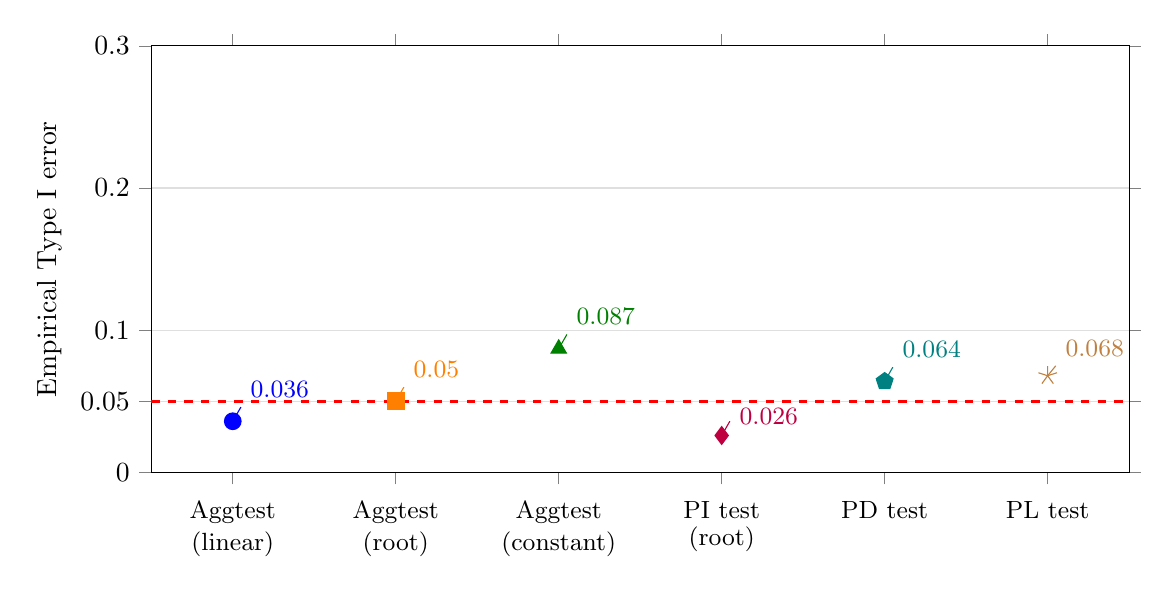
\begin{tikzpicture}

\begin{axis}[
width=14cm,
height=7cm,
ymin=0,
ymax=0.30,
ytick={0,0.05,0.1,0.2,0.3},
yticklabels={$0$,$0.05$,$0.1$,$0.2$,$0.3$},
scaled y ticks=false,
ylabel={Empirical Type I error},
xmin=0.5,
xmax=6.5,
xtick={1,2,3,4,5,6},
xticklabels={
{\shortstack{Aggtest\\(linear)}},
{\shortstack{Aggtest\\(root)}},
{\shortstack{Aggtest\\(constant)}},
{\shortstack{PI test\\(root)}},
{PD test},
{PL test}
},
x tick label style={font=\small,align=center,yshift=-1mm},
tick align=outside,
ymajorgrids=true,
grid style={gray,opacity=0.25},
clip=false
]

% Nominal significance level
\addplot[
red,
dashed,
very thick,
domain=0.5:6.5
] {0.05};

%==================================================
% Aggtest (linear)
%==================================================
\addplot[
only marks,
mark=*,
mark size=3pt,
blue
] coordinates {(1,0.036)};

\draw[blue,thin]
(axis cs:1,0.036) -- (axis cs:1.05,0.046);

\node[
blue,
font=\small,
anchor=south west
] at (axis cs:1.05,0.046) {0.036};

%==================================================
% Aggtest (root)
%==================================================
\addplot[
only marks,
mark=square*,
mark size=3pt,
orange
] coordinates {(2,0.050)};

\draw[orange,thin]
(axis cs:2,0.050) -- (axis cs:2.05,0.060);

\node[
orange,
font=\small,
anchor=south west
] at (axis cs:2.05,0.060) {0.05};

%==================================================
% Aggtest (constant)
%==================================================
\addplot[
only marks,
mark=triangle*,
mark size=3.2pt,
green!50!black
] coordinates {(3,0.087)};

\draw[green!50!black,thin]
(axis cs:3,0.087) -- (axis cs:3.05,0.097);

\node[
green!50!black,
font=\small,
anchor=south west
] at (axis cs:3.05,0.097) {0.087};

%==================================================
% PI test (root)
%==================================================
\addplot[
only marks,
mark=diamond*,
mark size=3.2pt,
purple
] coordinates {(4,0.026)};

\draw[purple,thin]
(axis cs:4,0.026) -- (axis cs:4.05,0.036);

\node[
purple,
font=\small,
anchor=south west
] at (axis cs:4.05,0.027) {0.026};

%==================================================
% PD test
%==================================================
\addplot[
only marks,
mark=pentagon*,
mark size=3.2pt,
teal
] coordinates {(5,0.064)};

\draw[teal,thin]
(axis cs:5,0.064) -- (axis cs:5.05,0.074);

\node[
teal,
font=\small,
anchor=south west
] at (axis cs:5.05,0.074) {0.064};

%==================================================
% PL test
%==================================================
\addplot[
only marks,
mark=star,
mark size=3.5pt,
brown
] coordinates {(6,0.068)};

\draw[brown,thin]
(axis cs:6,0.068) -- (axis cs:6.05,0.075);

\node[
brown,
font=\small,
anchor=south west
] at (axis cs:6.05,0.075) {0.068};

\end{axis}

\end{tikzpicture}

\end{document}